% ----------------------------------------------------------------------------------------------------- %
% Capítulo 6 - RESULTADOS
% ----------------------------------------------------------------------------------------------------- %
\chapter{Resultados Preliminares}
\label{cap:resultados}
\noindent No presente capítulo são descritos os resultados parciais qualitativos e quantitativos obtidos no decorrer da aplicação do questionário de avaliação do aprendizado dos estudantes da disciplina de Álgebra Linear que não estão utilizando a plataforma AlfaGebra.

\section{Disciplina Álgebra Linear}
\label{disciplina_3_ultimos_semestre}

\noindent Dados fornecidos pela professora da disciplina de Álgebra Linear, mostram que existem uma percentagem muito elevada de alunos evadidos no decorrer de cada semestre. Obtendo como base os três últimos semestre, 2015-2, 2016-1 e 2016-2, observa-se um número elevado de alunos que são reprovados por faltas como demonstrado na tabela \ref{dados_tres_semestres_alunos_algebra} que além de demonstrar os reprovados por faltas, mostra também a quantidade dos que foram aprovados por notas e reprovados por notas. É importante salientar que conforme a professora da disciplina, os acadêmicos já começam a evadir, logo após a aplicação da primeira avaliação. Estabelecendo uma média em relação a esses semestres, apresenta-se uma porcentagem de aproximadamente 47,06\% de alunos que são evadidos da disciplina, um dado que corresponde a quase metade dos alunos.
\begin{table}[!htp]
    \centering
    \begin{tabular}{lcccl}
                                                                            & \multicolumn{1}{l}{}                                         & \multicolumn{1}{l}{}                                         & \multicolumn{1}{l}{}                                         &  \\
                                                                            & \multicolumn{1}{l}{}                                         & \multicolumn{1}{l}{}                                         & \multicolumn{1}{l}{}                                         &  \\ \cline{1-4}
\multicolumn{1}{|l|}{}                                                      & \multicolumn{3}{c|}{\textbf{PERÍODO}}                                                                                                                                                      &  \\ \cline{2-4}
\multicolumn{1}{|l|}{\multirow{-2}{*}{}}                                    & \multicolumn{1}{c|}{\cellcolor[HTML]{EFEFEF}\textbf{2015-2}} & \multicolumn{1}{c|}{\cellcolor[HTML]{EFEFEF}\textbf{2016-1}} & \multicolumn{1}{c|}{\cellcolor[HTML]{EFEFEF}\textbf{2016-2}} &  \\ \cline{1-4}
\multicolumn{1}{|c|}{\textbf{Matriculados}}                                 & \multicolumn{1}{c|}{38}                                      & \multicolumn{1}{c|}{40}                                      & \multicolumn{1}{c|}{41}                                      &  \\ \cline{1-4}
\multicolumn{1}{|c|}{\cellcolor[HTML]{EFEFEF}\textbf{Aprovados}}            & \multicolumn{1}{c|}{\cellcolor[HTML]{EFEFEF}10}              & \multicolumn{1}{c|}{\cellcolor[HTML]{EFEFEF}20}              & \multicolumn{1}{c|}{\cellcolor[HTML]{EFEFEF}15}              &  \\ \cline{1-4}
\multicolumn{1}{|c|}{\textbf{Reprovados por faltas}}                        & \multicolumn{1}{c|}{21}                                      & \multicolumn{1}{c|}{12}                                      & \multicolumn{1}{c|}{23}                                      &  \\ \cline{1-4}
\multicolumn{1}{|c|}{\cellcolor[HTML]{EFEFEF}\textbf{Reprovados por notas}} & \multicolumn{1}{c|}{\cellcolor[HTML]{EFEFEF}7}               & \multicolumn{1}{c|}{\cellcolor[HTML]{EFEFEF}8}               & \multicolumn{1}{c|}{\cellcolor[HTML]{EFEFEF}3}               &  \\ \cline{1-4}
\end{tabular}
    \caption{Dados dos quantitativos de alunos nos três últimos semestres, referentes a aprovados por notas, reprovados por faltas e reprovados por notas}
    \label{dados_tres_semestres_alunos_algebra}
\end{table}

A tabela \ref{algebra_linear_2015_2} demonstra os resultados da disciplina de Álgebra Linear no semestre de 2015-2, em relação ao quantitativo de alunos que foram aprovados, reprovados por faltas e reprovados por notas, ao qual nesse período a citada disciplina apresentava um total de 38 alunos e dentre esses, apenas 26,32\% foram os aprovados por notas, 55,26\% reprovados por faltas e 18,42\% reprovados por notas.

\begin{figure}[!htb]
  \centering 
  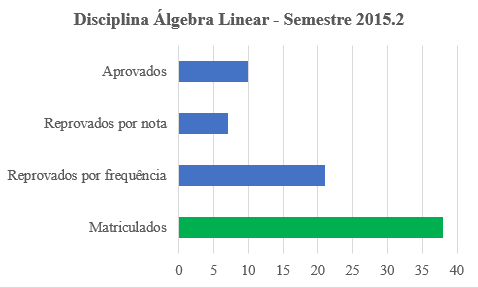
\includegraphics[scale=1]{Figuras/2015-2.png}
  \caption{Dados dos alunos referente a disciplina de Álgebra Linear no semestre 2015-2}\label{algebra_linear_2015_2}
\end{figure}

Em relação ao semestre de 2016-1, na figura \ref{algebra_linear_2016_1} são destacados o quantitativo referente ao semestre em questão, em que dentre as 3 (três) categorias, aprovados, reprovados por notas e reprovados por faltas, são destacados os seguintes dados obtidos perante a análise do gráfico: aprovados por notas cerca de 50\%, reprovados por notas 20\% e reprovados por faltas 30\%.

\begin{figure}[!htb]
  \centering 
  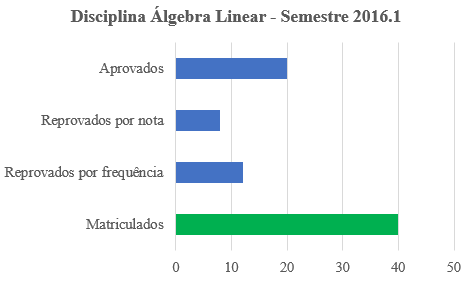
\includegraphics[scale=1]{Figuras/2016-1.png}
  \caption{Dados dos alunos referente a disciplina de Álgebra Linear no semestre 2016-1}\label{algebra_linear_2016_1}
\end{figure}

Por fim, no semestre de 2016-2, a figura \ref{algebra_linear_2016_2} mostra que mais da metade dos estudantes ficaram como reprovados por faltas, sendo 56,10\% e os demais referem-se aos reprovados por notas com um total de 7,32\% e aprovados por notas com 36,58\%.

\begin{figure}[!htb]
  \centering 
  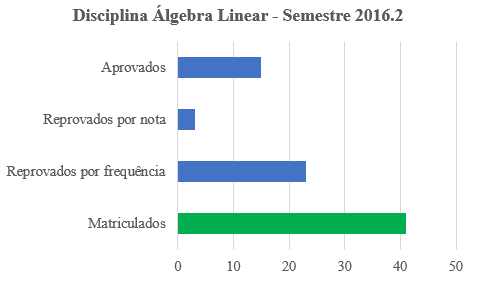
\includegraphics[scale=1]{Figuras/2016-2.png}
  \caption{Dados dos alunos referente a disciplina de Álgebra Linear no semestre 2016-2}\label{algebra_linear_2016_2}
\end{figure}

A partir desses dados é possível verificar que os índices de reprovações da disciplina nos três últimos semestres correspondem a 16,51\% e esse dado não é tão elevado, mas considerando o total de 51,37\% referente aos reprovados por faltas, esses dados poderiam ser diferentes devido ao alto nível de abstração que a disciplina apresenta, por conseguinte, muitos deles desistem.

\section{Coleta de dados}
\label{coleta_dados}

\noindent Com objetivo de investigar por que os acadêmicos da disciplina de Álgebra Linear sentem desmotivados no estudo da Álgebra Linear, as dificuldades encontradas em absorver os conteúdos da disciplina e a importância da aplicação de recursos tecnológicos para o aprendizado foi desenvolvido um questionário base estruturado como previsto na metodologia e aplicado para a turma de Álgebra Linear do semestre de 2017-1, no curso de Ciência da Computação, o qual foi aplicado no dia 19 de outubro de 2017 e apresentava perguntas objetivas de múltiplas escolhas e discursivas. A aplicação foi direcionada para um total de 40 alunos, em conformidade com o número de matriculados na disciplina, mas no dia da aplicação encontravam-se somente 22 (vinte e dois) acadêmicos presente na sala de aula e é importante salientar que já havia sido aplicada a primeira avaliação.  

Com o questionário foi possível identificar o grau de dificuldade da disciplina de acordo com os acadêmicos, a qual a figura \ref{grau_dificuldade} explana os dados obtidos e que de um total de 22 alunos que participaram da pesquisa 40,90\% consideraram a disciplina com grau de dificuldade alto, 50\% como médio, 9,10\% sendo razoável e nenhum estudante achou a disciplina fácil e os estudantes relataram que dentre os conteúdos presente na estrutura curricular da disciplina o mais difícil de absorver é espaço vetorial. Um ponto a destacar é que alguns alunos chegam no ensino superior muitas vezes despreparados em alguns assuntos da matemática o que muitas vezes torna um ponto difícil no início do estudo da Álgebra Linear e não somente nela mais também nas demais disciplinas de cálculos.

\begin{figure}[!htb]
  \centering 
  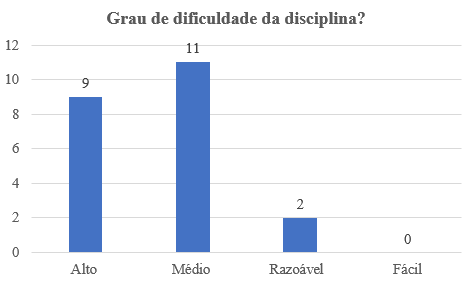
\includegraphics[scale=1]{Figuras/grau_dificuldade.png}
  \caption{Grau de dificuldade dos alunos}\label{grau_dificuldade}
\end{figure}
 
Diante dos resultados demonstrados referente ao grau de dificuldade, buscou-se entender qual é a maior dificuldade no aprendizado da Álgebra Linear e cerca de 45,45\% dos estudantes relataram que a maior dificuldade encontrada é em relação o alto nível de abstração, e para contornar esse alto nível, os acadêmicos utilizam como métodos de estudo, listas de exercícios e a maioria gosta de estudar individualmente. Vale salientar que a assiduidade com que os acadêmicos procuram o professor para sanar suas dúvidas relativas à disciplina é ínfima, a figura \ref{frequencia_procura_professor} evidencia esse dados, sendo que apenas 4,54\% dos estudantes já o procuraram nesse semestre, em condição razoavelmente, 36,36\% procuram às vezes e 54,54\% nunca procuraram.

\begin{figure}[!htb]
  \centering 
  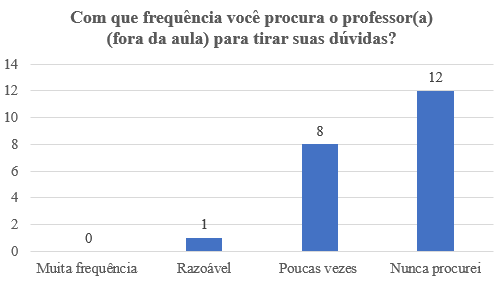
\includegraphics[scale=1]{Figuras/frequencia_professor.png}
  \caption{Frequência que os alunos procuram o professor}\label{frequencia_procura_professor}
\end{figure}

Um dado importante a ser destacado é a quantidade de vezes que o estudante está realizando a disciplina, pois este remete aos índices de reprovações e o grau de dificuldade enfrentado durante o estudo. Para esse dado, a figura \ref{numero_alunos_cursaram_vezes} mostra que 31,81\% estão realizando pela a segunda vez e 9,10\% pela terceira vez.

\begin{figure}[!htb]
  \centering 
  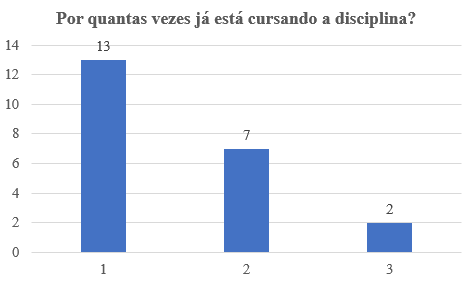
\includegraphics[scale=1]{Figuras/cursada_vezes.png}
  \caption{Quantitativo de alunos que cursaram a disciplina de Álgebra Linear}\label{numero_alunos_cursaram_vezes}
\end{figure}

Em relação ao uso de tecnologias para auxiliar no aprendizado dos conteúdos, 81,81\% dos estudantes relataram que se fosse disponibilizado algum recurso tecnológico para auxiliar no estudo/aprendizado da Álgebra Linear eles utilizariam, além dos estudantes que relataram que a utilizaria, nenhum estudante comentou que a não utilizaria, mas 18,18\% ficaram indecisos na escolha se a utilizaria ou não. Contudo, demonstraram que a ideia desse recurso tecnológico é excelente, pois ajudaria a entender os conteúdos e que seria uma nova metodologia tecnológica, na figura \ref{tecnologia_estudo} esses dados estão representados graficamente. 

No que concerne a utilização do sistema AlfaGebra, 100\% dos alunos responderam que utilizariam no decorrer dos estudos e seria uma ferramenta útil para o aprendizado e que 86,36\% relataram que a utilização desse sistema no decorrer das aulas possibilitaria maior dinamismo.

\begin{figure}[!htb]
  \centering 
  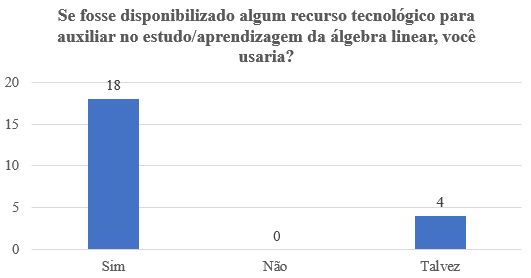
\includegraphics[scale=1]{Figuras/tecnologia_usa.png}
  \caption{Utilização de tecnologias para o estudo}
  \label{tecnologia_estudo}
\end{figure}

